\documentclass{standalone}
\usepackage{tikz}
\usepackage{ctex,siunitx}
\setCJKmainfont{Noto Serif CJK SC}
\usepackage{tkz-euclide}
\usepackage{amsmath}
\usetikzlibrary{patterns, calc}
\usetikzlibrary {decorations.pathmorphing, decorations.pathreplacing, decorations.shapes,}

\begin{document}
\small
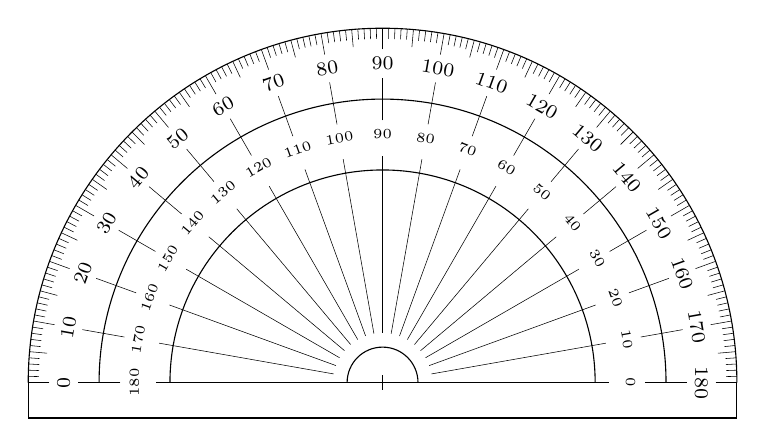
\begin{tikzpicture}[>=stealth,scale=0.9]
  \tkzSetUpPoint[fill=black]
  % \useasboundingbox(-1,-0.75)rectangle(3.7,1.4);
  \draw(-5,0) --(-5,-0.5) --(5,-.5)--(5,0);	
  \foreach \x in {.5, 3.0,4.0,5}
    {
      \draw[thin](\x ,0) arc (0:180:\x );
    }
  \foreach \x in {0, 10,20,...,170,180}
    {
      \draw[very thin] (\x:0.7)--(\x:3.2);
      \draw[very thin] (\x:3.7)--(\x:4.3);
      \draw[very thin] (\x:4.7)--(\x:5);
      \node[rotate=-90+\x] at (\x:3.5){\tiny \x};
      \node[rotate=90-\x] at (180-\x:4.5){\scriptsize \x};
    }
  \foreach \x in {0, 10,20,...,170}
    {
      \foreach \y in {1,2,3,4,6,7,8,9}
        {
          \draw[very thin] (\x+\y:4.85)--(\x+\y:5);
        }
      \draw[very thin] (\x+5:4.75)--(\x+5:5);
    }
  \draw[very thin](-0.7,0)--(0.7,0)(0,0.1)--(0,-0.1);
\end{tikzpicture}
\end{document}